\section{Architecture}

A program can be represented in several ways. There is extensive reading material on how logical programming can be used to represent and analyse programs\cite{Reps1995}\cite{DatalogDBQueries}. However, other approaches exist that lean more closely towards the implementation of our system.  As discussed in section \ref{subsec:staticAnalysis}, static analysis can be a means of representing implicit and explicit information about a piece of source code. For our approach, we needed a representation containing enough information to look up non-trivial properties about how information and data flows in the program. Abstract interpretation of a program produces an abstract state graph that meets these requirements. The graph contains information about control- and data flow, providing a rich source of information that can be extracted through some query language and a querying mechanism. 

% Querying mechanisms -> approaches in datalog queries enzo
Querying programs depends greatly on the way a program is represented and how queries are transformed into query-engine-friendly data structures. One way would be to resolve queries using existing techniques such as \cite{bddbddb}. This technique matches queries expressed in Datalog against a database of rules representing the relations of an entire program. Since our approach represents programs as flow graphs, an alternative method to resolve queries needs to be applied. A suitable algorithm to solving queries is presented in \cite{algoEngine}, which enables us to query flow graphs directly. The internals of this algorithm will be discussed in greater detail in section \ref{subsec:matchingEngine}.

% DSL
It is important that exploring and accessing information of a flow graph happens in an easy and user-friendly way. We believe regular path expressions to be the most legible way to write clean and understandable queries. With the JS-QL language, we offer an internal domain-specific language specialized in expressing queries corresponding to sequences of states in the flow graph. 

The actual architecture of the JS-QL framework is depicted in figure \ref{fig:architecture}. The query engine takes as input (i) a flow graph and (ii) a query, written in the JS-QL language. The output will consist of tuples \texttt{<State, Substitutions>} for all paths on which a match for the query was found.

\begin{figure}
    \centering
      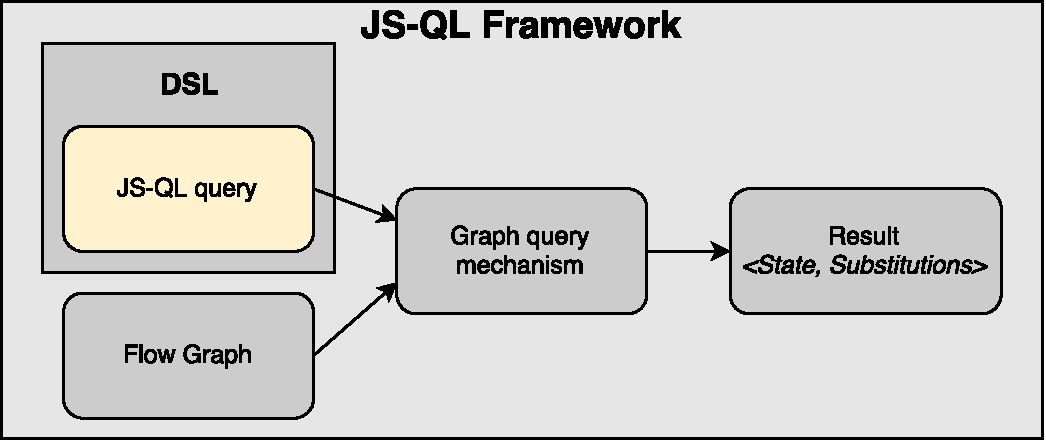
\includegraphics[width=0.9\textwidth]{images/Architecture} 
      \caption{JS-QL framework architecture}
    \label{fig:architecture}
\end{figure}
\section{Flow graphs for JavaScript programs}

The need for detailed control- and data flow information in our program representation graph limits the types of graphs that can be used for our framework. Program dependence graphs\cite{PDG} for example can be very useful to track the flow of information between certain points in a program but often lack more general information about program states, making them less qualified to use as our main program representation. In contrast, the JIPDA\cite{} abstract state graph contains all the information needed to precisely express patterns to be detected in a program. This section takes an in-depth look at the JIPDA abstract state graph and the information it holds in its states. Figure \ref{fig:JipdaGraph} shows part of a typical graph produced by JIPDA for a program containing a check for whether a number is equal to zero or not.

As can be observed, the graph depicts all possible paths a program can traverse. Since the analysis in JIPDA is flow-sensitive, it is guaranteed that a state \texttt{a} on some path in the graph occurs before a state \texttt{b} on the same path if state \texttt{a} occurs first before state \texttt{b} on the path. This makes reasoning about patterns in a program much easier, since no false positives will occur with regards to the order of execution of states. The graph produced by the JIPDA analysis is also a flow graph, and more precisely maintains information about two types of flows:
%TODO uitleggen flow graph value flow en control flow -> in JIPDA

\begin{enumerate}
\item \textit{data flow}: Information about what values an expression may evaluate to.
\item \textit{Control flow}: Information about which functions can be applied at a call site.
\end{enumerate}

We need these kinds of information to be able to make correct assumptions at certain states in a program. Consider the expression \texttt{f(x)} for example. Function \texttt{f} will be the function that is invoked. The value of \texttt{f} however may depend on other operations that occur before this function call, such as another function call. Therefore it is important to know which function(s) \texttt{f} may refer to, illustrating the need of control and data flow.

\subsection*{States of an abstract state graph}

The abstract state graph is an alternation of four different types of states. JIPDA internally uses Esprima\cite{Esprima} to parse JavaScript code and set up an abstract syntax tree (AST). This AST is the starting point for the analysis that JIPDA performs, hence information about the nodes from the AST is also contained in certain states in the resulting graph. These states are marked in red and are so-called \textit{evaluation states}. Other states are \textit{continuation states} (green), \textit{return states} (blue) and \textit{result states} (yellow).

\begin{figure}[!ht]
    \centering
      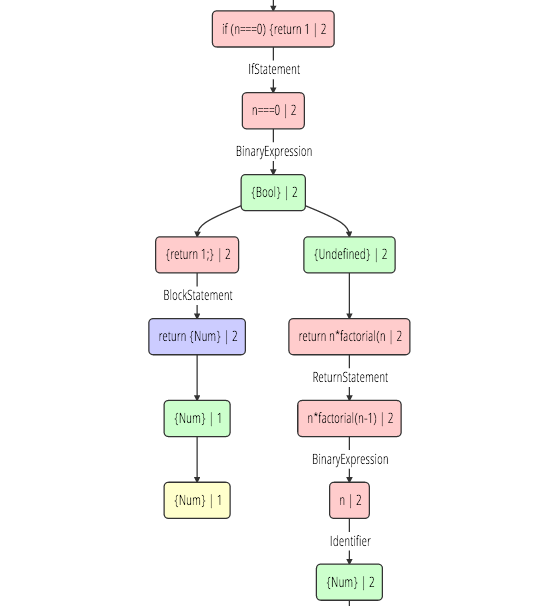
\includegraphics[width=262px, height=606px, keepaspectratio]{images/JipdaGraph} 
      \caption{Example JIPDA abstract state graph}
    \label{fig:JipdaGraph}
\end{figure}

%HELP VRAGEN BIJ JENS
\begin{enumerate}
\item \textit{Evaluation state}: Represents the evaluation of an expression or statement in the program.
\item \textit{Continuation state}: ...
\item \textit{Return state}: Indicates the return of a function application, having the returned value stored in one of its properties.
\item \textit{Result state}: Final state of the graph, indicating the abstract final value(s) of the program. The graph can have more than one result state, depending on the program's nature. 
\end{enumerate}

These states all contain valuable information about the point in the program they represent. The next part of this section discusses the different attributes that can be found in the states of the abstract state graph. 

%Kont, Lkont, Node, Benv, Store, Value
\subsection*{Node}

As said earlier, evaluation states contain information about the expression or statement they represent in the program. This information is stored in the form of an AST node, as obtained by the Esprima parser. Detailed information about the current expression or statement can be found in the properties of these nodes. Our approach makes extensive use of this information to find a match for a specified pattern along the graph. Note that node information is exclusively available in evaluation states. If we parse the following program \\\\
\texttt{function answerToTheUniverse(arg)\{}\\
\phantom{ }\phantom{ }\phantom{ }\phantom{ }\texttt{return 42;}\\
\texttt{\}}\\
\\
we obtain its corresponding JSON representation, listed in \ref{lst:EsprimaTree}.
\\
\begin{lstlisting}[label={lst:EsprimaTree},language=JSON,caption=Parsed JavaScript program AST, mathescape=true]  % float=t?

{
    "type": "Program",
    "body": [
        {
            "type": "FunctionDeclaration",
            "id": {
                "type": "Identifier",
                "name": "answerToTheUniverse"
            },
            "params": [
                {
                    "type": "Identifier",
                    "name": "arg"
                }
            ],
            "defaults": [],
            "body": {
                "type": "BlockStatement",
                "body": [
                    {
                        "type": "ReturnStatement",
                        "argument": {
                            "type": "Literal",
                            "value": 42,
                            "raw": "42"
                        }
                    }
                ]
            },
            "generator": false,
            "expression": false
        }
    ]
}
\end{lstlisting}

The parsed source code is a list of nodes contained in the body property of the "program" AST node. This is in fact the root node of the AST. Each node has its own \textit{type} that distinguishes different kinds of expressions and statements. The example code in \ref{lst:EsprimaTree} shows that the parsed code is a "FunctionDeclaration" with its own id, parameters, defaults and body attributes. We observe that the attributes in turn can again be (a list of) nodes.

\subsection*{Binding environment and store}

In JIPDA, variables point to addresses. The mapping of a variable to an address is called a \textit{binding}. These bindings reside in a \textit{binding environment $\hat{\beta}$}. Each binding maps to a value through the \textit{store} $\hat{\sigma}$. The store acts as a heap where bindings represent addresses on that heap. Being able to capture bindings, addresses and values in metavariables enables us to express and inspect data flow properties of programs. Variables are mapped to values in two stages. The first step for looking up a variable $\hat{\nu}$ is to locate its binding in $\hat{\beta}$. Next, the value of the variable can be looked up in the store by composing these two functions. The value of $\hat{\nu}$ is given by $\hat{\sigma}(\hat{\beta}(\hat{\nu}))$. This way of mapping variables to values allows us to reason about individual bindings, which is necessary because during interpretation multiple bindings to the same variable can exist simultaneously. Listing \ref{lst:benvStoreExample} gives an example of how a variable gets a binding and is later looked up.
\\
\begin{lstlisting}[label={lst:benvStoreExample},language=JavaScript,caption=Example of the binding environment and store workings, mathescape=true]  % float=t?

function f(){
  //$\hat{\beta}$ contains a binding $x \rightarrow \widehat{Addr}$
  var x = 3; 
  
  //$\hat{\sigma}$ has an entry $\widehat{Addr} \rightarrow \widehat{Val}$
  //and the (set of) corresponding value(s) for x is returned. 
  return x;
}
var value = f();
\end{lstlisting}


\subsection*{Value}
%Value uit store
The lookup of a variable through a binding in the store results in the (set of) value(s) for that variable. This information is available in all states but evaluation states. For continuation states, the value will represent the looked up or calculated values of an expression. A return state's value is the set of possible values that will be returned. Result states contain the final values of a program.

\subsection*{Application context}

Some text about the application context.

\subsection*{Stack}

Some text about the stack.




\section{External DSLs for querying graphs}
%Intro http://www.st.ewi.tudelft.nl/~arie/papers/dslbib.pdf

\subsection{Domain-specific language vs general purpose language}
%Wat is een DSL & wat is een GPL

%A domain-specific language (DSL) is a programming language or executable specification language that offers, through appropriate notations and abstractions, expressive power focused on, and usually restricted to, a particular problem domain. 
%Key is focussed expressive power

%  Many DSLs are supported by a DSL compiler which generates applications from DSL programs. In this case, the DSL compiler is referred to as application generator in the literature [17], and the DSL as application-specific language. Other DSLs, such as YACC [7] or ASDL [77], are not aimed at programming (specifying) complete applications, but rather at generating libraries or components. Also, DSLs exist for which execution consists in generating documents (TEX), or pictures (PIC [7]). A common term for DSLs geared towards building business data processing systems is 4th Generation Language (4GL). Related to domain-specific programming is end-user programming, which happens when end-users perform simple programming tasks using a macro or scripting language. A typical example is spreadsheet programming using the Excel macro-language.
%Why a DSL 	-> Bentley1986 
%			-> reusability : http://www.biglever.com/papers/Krueger_AcmReuseSurvey.pdf
%advantages/disadvantages DSL -> http://www.st.ewi.tudelft.nl/~arie/papers/dslbib.pdf

%https://pdfs.semanticscholar.org/72ec/5c5000ee860d1ed28a4a91100ac91a3c7afe.pdf

%\subsection{Internal DSLs} -> MOET DIT?
%eerste keer door Hudak -> http://citeseerx.ist.psu.edu/viewdoc/download?doi=10.1.1.49.6020&rep=rep1&type=pdf
% Embedded kan GPL gebruiken. -> Sometimes, however, they contain an entire general-purpose language (GPL) as a sublanguage, thus offering domain-specific expressive power in addition to the expressive power of the GPL. This situation occurs when DSLs are implemented as embedded languages
%Waarom internal
%----------------
%RW over DSEL graph traversal:
%http://arxiv.org/pdf/1508.03843.pdf -> Graph traversal
%-----------------------------
%RW over DSEL los van graphs:
%https://www.usenix.org/events/dsl99/full_papers/jennings/jennings.ps
%https://www.usenix.org/legacy/publications/library/proceedings/dsl97/full_papers/stevenson/stevenson.pdf
%http://haskell.cs.yale.edu/wp-content/uploads/2011/02/padl99.pdf
%Eliott1999
%https://www.usenix.org/legacy/publications/library/proceedings/dsl97/full_papers/kamin/kamin.pdf
%-----------------------------

%2 die ik al had -> 1 ervan queriet graphs!

%https://idl.cs.washington.edu/files/2014-Ellipsis-EuroVis.pdf --> Zij doen wel element van fluent API als argument -> Overwegen of gebruiken of niet
% MISSCHIEN http://www.cs.um.edu.mt/gordon.pace/Research/Papers/wict2009-01.pdf



\subsection{External DSLs}

%Waarom external
%RW over EDSL graph traversal:
%StruQL -> downloads file35
%http://infolab.stanford.edu/lore/pubs/lorel96.pdf -> Semistructured data
%http://www.cs.nyu.edu/~lharris/papers/crew.pdf -> Trees
%http://sites.fas.harvard.edu/~cs265/papers/he-2008.pdf -> GraphQL
%-----------------------------
%RW over EDSL los van graphs:
%http://graphics.stanford.edu/hackliszt/liszt_sc2011.pdf
%http://homepages.cwi.nl/~jurgenv/papers/SCAM-2009.pdf
%https://www.researchgate.net/publication/220071161_BDL_A_Specialized_Language_for_Per-Object_Reactive_Control
%Chandra1999
%http://citeseerx.ist.psu.edu/viewdoc/download?doi=10.1.1.29.9540&rep=rep1&type=pdf -> saaiste shit ever
%-----------------------------


\section{Design of an internal DSL for querying flow graphs}

%zie Domain-specific languages: An annotated Bibliography

%Waarom internal (als niet besproken in section hiervoor)

\subsection{internal DSL design constraints}

%CONSTRAINTS:
% What is the problem domain? -> Domein afbakenen kan via http://citeseerx.ist.psu.edu/viewdoc/download?doi=10.1.1.49.9877&rep=rep1&type=pdf
%Flow graphs beperken predikaten, Extensibility, JavaScript, no REPL
%https://idl.cs.washington.edu/files/2014-Ellipsis-EuroVis.pdf --> Zij doen wel element van fluent API als argument -> Overwegen of gebruiken of niet
\subsection{DSL implementation techniques}
%Welke bestaan er, welke hebben wij genomen

\subsection{DSL design patterns}
%Papers!

